%%%%%%%%%%%%%%%%%%%%%%%%%%%%%%%%%%%%%%%%%
% a0poster Portrait Poster
% LaTeX Template
% Version 1.0 (22/06/13)
%
% The a0poster class was created by:
% Gerlinde Kettl and Matthias Weiser (tex@kettl.de)
% 
% This template has been downloaded from:
% http://www.LaTeXTemplates.com
%
% License:
% CC BY-NC-SA 3.0 (http://creativecommons.org/licenses/by-nc-sa/3.0/)
%
%%%%%%%%%%%%%%%%%%%%%%%%%%%%%%%%%%%%%%%%%

%----------------------------------------------------------------------------------------
%	PACKAGES AND OTHER DOCUMENT CONFIGURATIONS
%----------------------------------------------------------------------------------------

\documentclass[a0,portrait]{a0poster}

\usepackage{multicol} % This is so we can have multiple columns of text side-by-side
\columnsep=100pt % This is the amount of white space between the columns in the poster
\columnseprule=3pt % This is the thickness of the black line between the columns in the poster

\usepackage[svgnames]{xcolor} % Specify colors by their 'svgnames', for a full list of all colors available see here: http://www.latextemplates.com/svgnames-colors

\usepackage{times} % Use the times font
%\usepackage{palatino} % Uncomment to use the Palatino font

\usepackage{graphicx} % Required for including images
\graphicspath{{figures/}} % Location of the graphics files
\usepackage{booktabs} % Top and bottom rules for table
\usepackage[font=small,labelfont=bf]{caption} % Required for specifying captions to tables and figures
\usepackage{amsfonts, amsmath, amsthm, amssymb} % For math fonts, symbols and environments
\usepackage{wrapfig} % Allows wrapping text around tables and figures
\usepackage{multirow}
\definecolor{darkgreen}{HTML}{00A000}
\definecolor{darkblue}{HTML}{0000A0}
\definecolor{darkred}{HTML}{D00000}
\usepackage[colorlinks=true]{hyperref}%%%%%%%%%[,backref]!!!!!!!!!!!!!!!!!!!!
\hypersetup{linkcolor=darkred, urlcolor=darkblue, citecolor=darkgreen}%%%%%%%%

\begin{document}

\newcommand{\rf}[1]{(\ref{#1})}
\newcommand{\RR}{\mathbb{R}}

%----------------------------------------------------------------------------------------
%	POSTER HEADER 
%----------------------------------------------------------------------------------------

% The header is divided into two boxes:
% The first is 75% wide and houses the title, subtitle, names, university/organization and contact information
% The second is 25% wide and houses a logo for your university/organization or a photo of you
% The widths of these boxes can be easily edited to accommodate your content as you see fit

\begin{minipage}[b]{0.75\linewidth}
\veryHuge \color{NavyBlue} \textbf{Numerical Study of Soliton Solutions to the Two Dimensional Boussinesq  Equation} \color{Black}\\ % Title
%\Huge\textit{An Exploration of Complexity}\\[2cm] % Subtitle
\huge \textbf{K. Angelow \& N. Kolkovska}\\[0.5cm] % Author(s)
\huge Bulgarian Academy of Sciences, Institute of Mathematics and Informatics\\[0.4cm] % University/organization , ul. Acad. G. Bonchev, block 8, 1113 Sofia, Bulgaria
\Large \texttt{angelow@math.bas.bg, n.kolkovska@gmail.com}\\
\end{minipage}
%
\begin{minipage}[b]{0.25\linewidth}

\includegraphics[width=20cm]{Logo_Bulgaria.png}\\
\end{minipage}

\vspace{1cm} % A bit of extra whitespace between the header and poster content

%----------------------------------------------------------------------------------------

\begin{multicols}{2} % This is how many columns your poster will be broken into, a portrait poster is generally split into 2 columns

%----------------------------------------------------------------------------------------
%	ABSTRACT
%----------------------------------------------------------------------------------------

\color{Navy} % Navy color for the abstract

\begin{abstract}

This paper evaluates propagating wave solutions to the two dimensional Boussinesq Equation (BE). High order finite difference schemes for the spatial derivatives are implemented to solve this nonlinear hyperbolic problem. Taylor Series (TS) expansion method about time is used to move the solution forward. An explicit formula for boundary Conditions (BC) is applied on the computational boundary. The resulting numerical method has high accuracy of second, fourth and sixth order both in space and time. The performed numerical tests exhibit good convergence and confirm the validity of the TS method. Furthermore, the propagating wave preserves its maximum and more importantly, its shape.

\end{abstract}

%----------------------------------------------------------------------------------------
%	INTRODUCTION
%----------------------------------------------------------------------------------------

\color{SaddleBrown} % SaddleBrown color for the introduction

\section*{Introduction}

In this paper we  consider the two dimensional Boussinesq  Equation (BE)
\begin{align} \label{eq1}
&u_{tt} - \Delta u -\beta_1  \Delta u_{tt} +\beta_2 \Delta ^2 u + \Delta f(u)=0   \quad \text{for}  (x,y) \in \RR^2, \, t\in\RR^+, 
\\ \nonumber &u(x,y,0)=u_0(x,y), \, u_t(x,y,0)=u_1(x,y)   \quad\text{for} \, (x,y) \in \RR^2,
\\  &u(x,y) \rightarrow 0,  \Delta u(x,y) \rightarrow 0 ,  \quad \text{for}  \sqrt{x^2 + y^2} \rightarrow \infty, \label{eq11}
\end{align}
where $f(u)=\alpha u^2$,  $\alpha>0$, $\beta_1>0$, $\beta_2>0$  are dispersion parameters, and $\Delta$ is the Laplace operator. 

The BE is famous with the approximation of shallow water waves or also weakly non--linear long waves. It is often used for simulation of various physical processes e.g. turbulence in fluid mechanics, vibrations in acoustics, geotechnical engineering, atmosphere dynamics, etc. A derivation of the BE from the original Boussinesq system can be found in \cite{ChChr}.
%----------------------------------------------------------------------------------------
%	OBJECTIVES
%----------------------------------------------------------------------------------------

\color{DarkSlateGray} % DarkSlateGray color for the rest of the content

\section*{Main Objectives}

\begin{enumerate}
\item Investigate accurate solutions to \rf{eq1} with new initial and boundary conditions obtained in \cite{EllipticProblem}, \cite{BoundaryProblem}.
\item Show that the numerical solution converges over nested grids that are defined inside the equation domain $\Omega$.
\item Check the soliton properties of the solution, i.e. the solution wave is localized in a small region inside $\Omega$ and is of permanent form. 
\end{enumerate}

%----------------------------------------------------------------------------------------
%	METHODS
%----------------------------------------------------------------------------------------

\section*{Taylor Series Method}

Suppose we have functions $y$ and $f$ with the following properties
\begin{equation}
y:I \rightarrow \RR, \quad f:I \times \Omega \rightarrow \RR \nonumber
\end{equation}
where $y \in C^1(I,\RR)$ and $f$ is sufficiently smooth on $I \times \Omega$. Then, $f$ represent the phase space and $y$ is the unknown function to the differential equaiton:
\begin{equation}
\dot{y}(t) = f(t, y(t)).
\end{equation}
By repeated differentiation we can find each function $\frac{d^s}{dt^s}y(t) = \frac{d^{s-1}}{dt^{s-1}}f(t, y(t))$ and evaluate it at $t=t_0$ for each derivative.
The order $s$ formula for computing $y(t_n)=$ $y(t_{n-1}+h)$ using these functions, evaluated at $t=t_{n-1}$ and $y=y_{n-1}$, is
\begin{eqnarray}
y_n = y_{n-1} + h f(t_{n-1}, y_{n-1}) + \frac{h^2}{2!} \frac{d^2}{dt^2} f(t_{n-1}, y_{n-1}) + ... + \frac{h^s}{s!} \frac{d^s}{dt^s} f(t_{n-1}, y_{n-1}), &\nonumber\\ 
f_i(t_l, y_l), y_l(t_l), t_l \in \RR, 1 \leq l \leq n, 1 \leq i \leq s
\end{eqnarray}
where we already have the pair $(t_0, y_0)$ from the initial condition of the differential equation.

\section*{High Order Finite Difference Schemes (FDS)}
The spatial derivatives discretization  is made by using centered finite differences and extending the stencil:
\begin{equation}\label{fd}
u_{\widehat{xx},p}(x) :=  \frac{1}{h^2} \sum\limits_{i=-p/2}^{p/2} d_i u(x+ih),
\end{equation}
 Here $p$ is equal to $2$, $4$ or $6$.  The weights $d_i$ which are taken from \cite{forn} are  
 $ 1,-2,1$ for $p=2$, $-\frac{1}{12}, \frac{4}{3}, -\frac{5}{2}, \frac{4}{3}, -\frac{1}{12}$ for $p=4$ and  $\frac{1}{90}, -\frac{3}{20}, \frac{3}{2}, -\frac{49}{18}, \frac{3}{2}, -\frac{3}{20}, \frac{1}{90}$ for $p=6$. The approximation error of  formulae \rf{fd} is $O(h^p)$. Replacing the Laplace operator in \rf{eq1} by the discrete Laplacian 
$$ \Delta_{h,p} v_{i,j} := (v_{i,j})_{\widehat{xx},p} + (v_{i,j})_{\widehat{yy},p}$$ 
we obtain FDS with high approxima order $O(h^4)$ for $p=4$ and  $O(h^6)$ for $p=6$.

%----------------------------------------------------------------------------------------
%	RESULTS 
%----------------------------------------------------------------------------------------

\section*{Results}
The BE equation \rf{eq1} is examined for two sets of parameters $\beta$ and $c$ where $\alpha = 1$ is kept constant. The following test shows single solution wave with $\beta = 3$, $c = 0.52$, $\tau = 0.02$, $h = 0.1$ and $\Omega_h \times T_{\tau}$ $= [40, 40] \times [40, 80] \times [0, 40]$. The approximation order is $O(h^6 + \tau^6)$ and the time domain is increased four times compared to results in Table 1.

\begin{center}\vspace{0.4cm}
		\begin{tabular}{||c|l|ll|ll||}
			\hline
			\hline
      \multirow{2  }{*}{FDS}        & \multirow{2  }{*}{$h$, $\tau$}  & \multirow{2  }{*}{errors $E_i$in$L_2$}  &Conv.& \multirow{2  }{*}{errors $E_i$in$L_\infty$}  &Conv.  \\
	         &                    &                               & Rate   &                                        & Rate \\
   			\hline 
					\hline 
  $\beta=3$       &0.2, 0.02   &            &        &                  &      \\
      c=0.52   &0.1, 0.01   &~ 1.097302 &           &~1.170439      &       \\
     $O(h^2 + \tau^ 2)$ &0.05, 0.005 &~ 0.141356 &2.95  &~0.174157 & 2 .74       \\
			\hline 
   $\beta=3$        &0.2, 0.08   &            &        &                  &      \\
   c=0.52   &0.1, 0.04   &~ 0.310917 &           &~0.376470      &       \\
     $O(h^4+ \tau^4)$ &0.05, 0.02 &~ 0.021432 &3.85 &~0.023294 & 4.01        \\
			\hline 
  $\beta=3$               &0.2, 0.08   &            &        &                  &      \\
   c=0.52                  &0.1, 0.04       &~ 0.094731 &           &~0.126129      &       \\
     $O(h^6+ \tau^6)$ &0.05, 0.02 &~ 0.001756 &5.75    &~0.002004 & 5.97       \\
	   \hline
			\hline 
\end{tabular}
\captionof{table}{\color{Green} Convergence test for FDS with different approximation errors $O(h^{2} + \tau^2 )$, $O(h^{4} + \tau^4 )$ and $O(h^{6} + \tau^6 )$. Errors $E_i$ are measured in $L_2$ and $L_\infty$ norms}
\end{center}\vspace{0.4cm}

\begin{center}
%\begin{figure}[!htbp]
%	\centering
	\begin{minipage}[b]{0.30\linewidth}
		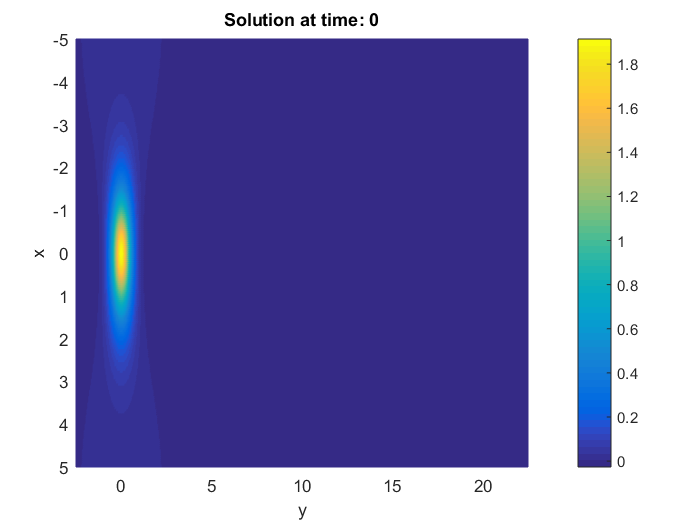
\includegraphics[width=\linewidth]{figures/Solution_bt3_t=0.png}
	\end{minipage}	
	\begin{minipage}[b]{0.30\linewidth}
		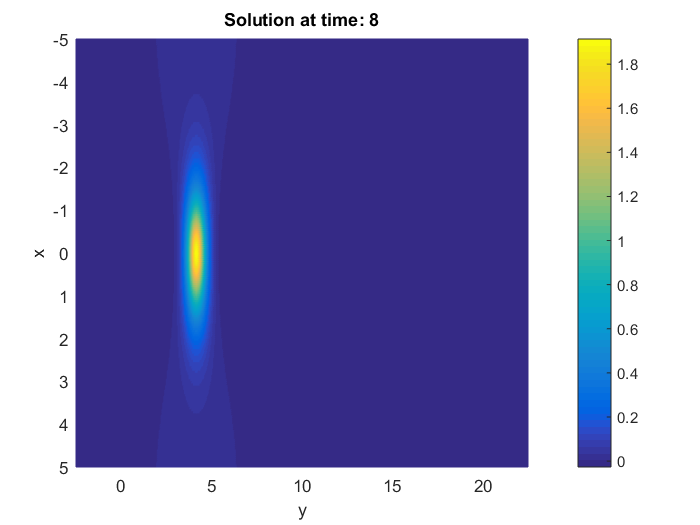
\includegraphics[width=\linewidth]{figures/Solution_bt3_t=8.png}
	\end{minipage}	
	\begin{minipage}[b]{0.30\linewidth}
		 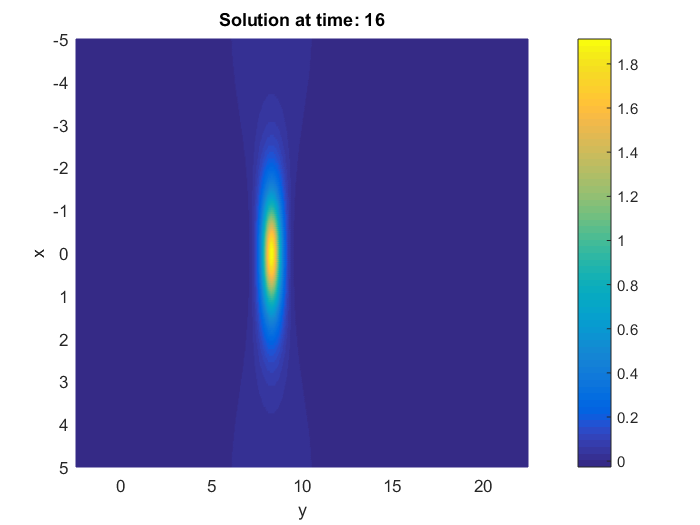
\includegraphics[width=\linewidth]{figures/Solution_bt3_t=16.png}
	\end{minipage}

	\begin{minipage}[b]{0.30\linewidth}
		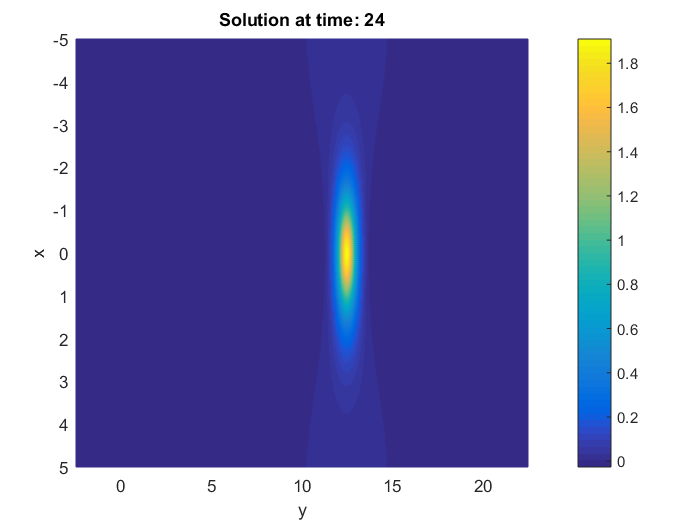
\includegraphics[width=\linewidth]{figures/Solution_bt3_t=24.png}
	\end{minipage}	
	\begin{minipage}[b]{0.30\linewidth}
		 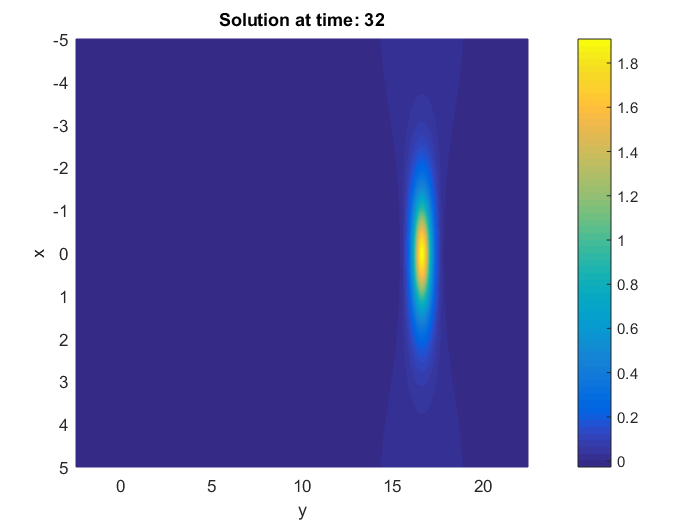
\includegraphics[width=\linewidth]{figures/Solution_bt3_t=32.png}
	\end{minipage}
	\begin{minipage}[b]{0.30\linewidth}
		 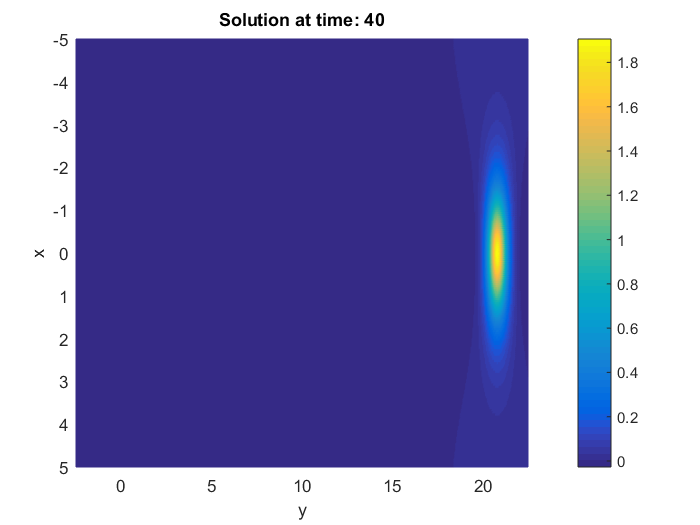
\includegraphics[width=\linewidth]{figures/Solution_bt3_t=40.png}
	\end{minipage}
	%\caption{Numerical solution of single wave for $\beta=3$ and $c = 0.52$ at times $t=0,8,16,24,32,40$.}
\captionof{figure}{\color{Green} Numerical solution of single wave for $\beta=3$ and $c = 0.52$ at times $t=0,8,16,24,32,40$.}
%\end{figure}
\end{center}\vspace{0.4cm}
The following test shows single solution wave with $\beta = 1$, $c = 0.9$, $\tau = 0.02$, $h = 0.1$ and $\Omega_h \times T_{\tau}$ $= [40, 40] \times [40, 80] \times [0, 40]$. The approximation order is $O(h^6 + \tau^6)$ and the time domain is increased four times compared to results in Table 2.

\begin{center}\vspace{0.8cm}
		\begin{tabular}{||c|l|ll|ll||}
			\hline
			\hline
      \multirow{2  }{*}{FDS}        & \multirow{2  }{*}{$h$, $\tau$}  & \multirow{2  }{*}{errors $E_i$in$L_2$}  &Conv.& \multirow{2  }{*}{errors $E_i$in$L_\infty$}  &Conv.  \\
	         &                    &                               & Rate   &                                        & Rate \\
   			\hline 
					\hline 
       $\beta=1$       &0.4, 0.02        &             &            &           &   \\
                  c=0.9    &0.2, 0.01       &~ 0.237432  &            &~0.097758 &   \\
  $O(h^2+ \tau^2)$ &0.1, 0.005   &~ 0.056544  &2.07  &~0.023651 & 2.04 \\
			\hline
      $\beta=1$    &0.4, 0.08    &            &            &             &    \\
       c=0.9 &0.2, 0.04    &~ 0.028098   &           &~0.013511  &   \\
       $O(h^4+ \tau^4)$ &0.1, 0.02   &~ 0.001801 & 3.96    &~0.000971  & 3.79  \\
    \hline
  $\beta=1$     &0.4, 0.08   &            &          &                  &      \\
      c=0.9    &0.2, 0.04   &~ 0.006722 &           &~0.003341      &       \\
     $O(h^6+ \tau^6)$ &0.1, 0.02 &~ 0.000137 &5.62  &~0.000070 & 5.58        \\
	   \hline
			\hline 
\end{tabular}
\captionof{table}{\color{Green} Convergence test for FDS with different approximation errors $O(h^{2} + \tau^2 )$, $O(h^{4} + \tau^4 )$ and $O(h^{6} + \tau^6 )$. Errors $E_i$ are measured in $L_2$ and $L_\infty$ norms}
\end{center}

%\begin{figure}[!htbp]
%	\centering
\begin{center}\vspace{0.4cm}
	\begin{minipage}[b]{0.30\linewidth}
		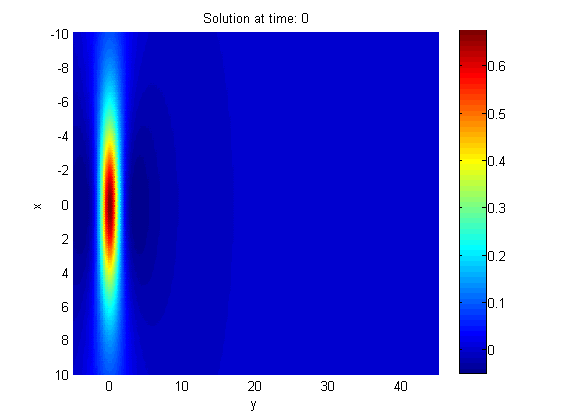
\includegraphics[width=\linewidth]{figures/Solution1_t=0.png}
	\end{minipage}	
	\begin{minipage}[b]{0.30\linewidth}
		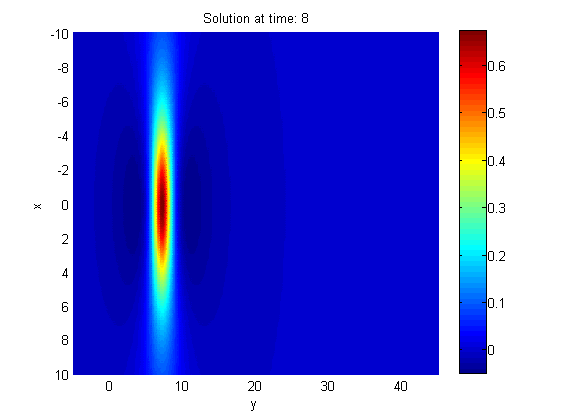
\includegraphics[width=\linewidth]{figures/Solution1_t=8.png}
	\end{minipage}	
	\begin{minipage}[b]{0.30\linewidth}
		 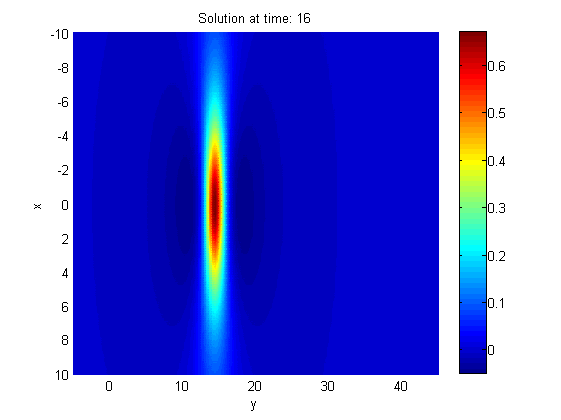
\includegraphics[width=\linewidth]{figures/Solution1_t=16.png}
	\end{minipage}
	\begin{minipage}[b]{0.30\linewidth}
		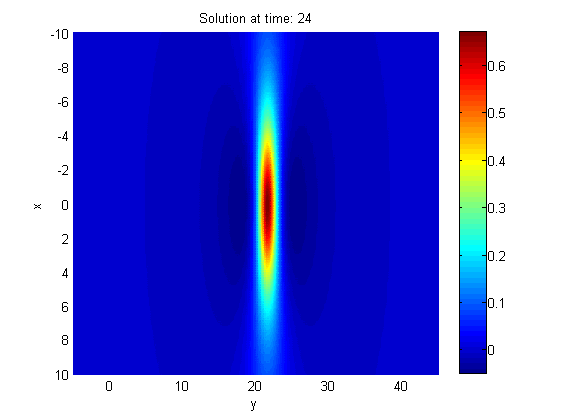
\includegraphics[width=\linewidth]{figures/Solution1_t=24.png}
	\end{minipage}	
	\begin{minipage}[b]{0.30\linewidth}
		 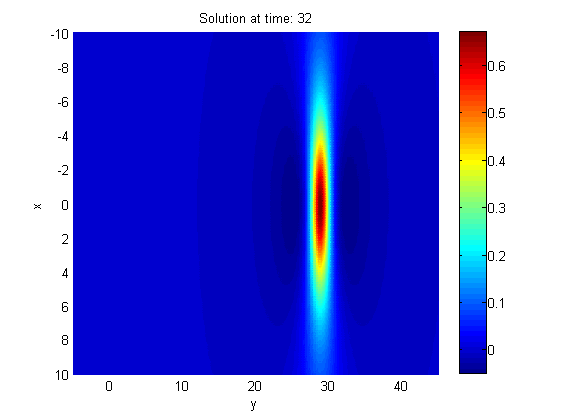
\includegraphics[width=\linewidth]{figures/Solution1_t=32.png}
	\end{minipage}
	\begin{minipage}[b]{0.30\linewidth}
		 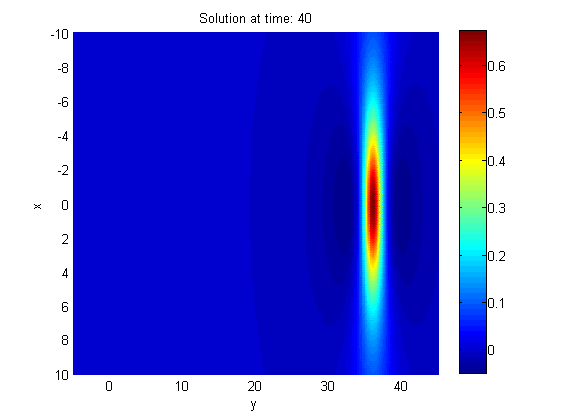
\includegraphics[width=\linewidth]{figures/Solution1_t=40.png}
	\end{minipage}
\captionof{figure}{\color{Green} Numerical solution of single wave for $\beta=1$ and $c = 0.9$ at times $t=0,8,16,24,32,40$.}
%	\caption{Numerical solution of single wave for $\beta=1$ and $c = 0.9$ at times $t=0,8,16,24,32,40$.}
%	\label{fig:oneWaveA}
%\end{figure}
\end{center}

Both waves behave like solitons, i.e. preserve shape and furthermore Figure 3 shows that the solutions have stable maxima.
\begin{center}\vspace{0.4cm}
	\begin{minipage}[b]{0.3\linewidth}
		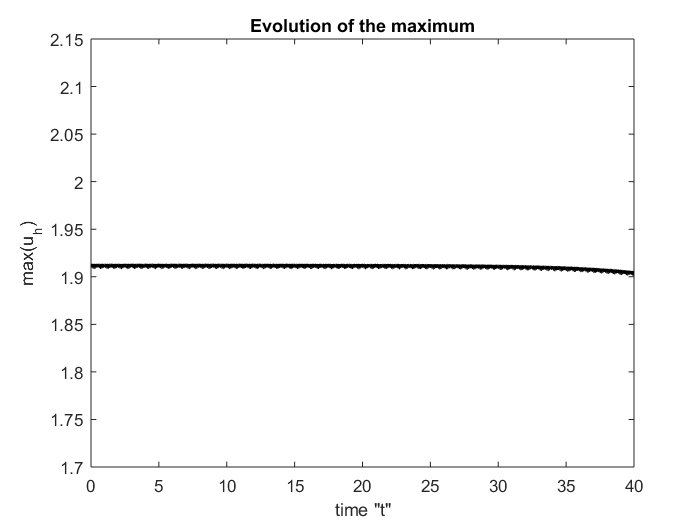
\includegraphics[width=\linewidth]{figures/EvolutionOfMaximum_bt3_t40.png}
	\end{minipage}	
	\begin{minipage}[b]{0.3\linewidth}
		 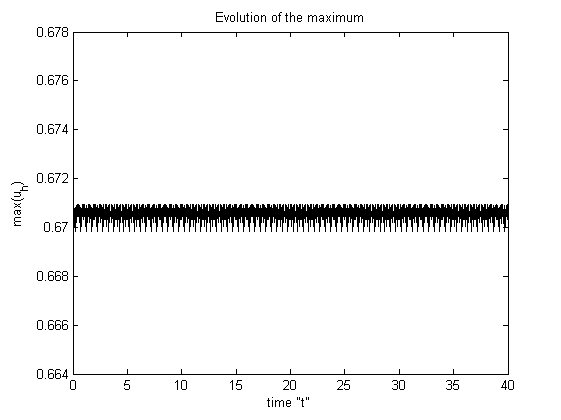
\includegraphics[width=\linewidth]{figures/EvolutionOfMaximum.png}
	\end{minipage}
\captionof{figure}{\color{Green} Evolution of the maximum for Test Wave $\beta =3$ (left panel) and $\beta=1$ (right panel).}
\end{center}
	%\caption{Evolution of the maximum for Test Wave $\beta =3$ (left panel) and $\beta=1$ (right panel).}

%----------------------------------------------------------------------------------------
%	CONCLUSIONS
%----------------------------------------------------------------------------------------

\color{SaddleBrown} % SaddleBrown color for the conclusions to make them stand out
\section*{Conclusions}

\begin{itemize}
\item Series of numerical experiments validate the numerical method. The results show that the approximate Taylor series method achieves the prescribed high accuracy. 
\item The resulting two numerical solutions for wave speeds near the upper limit $c_{max} $, $c < c_{max}$ are stable in form and  their maxima are changed for long period of time $T=40$ with small errors.  Thus the obtained solutions show soliton behavior. 
\end{itemize}
\color{DarkSlateGray} % Set the color back to DarkSlateGray for the rest of the content
%----------------------------------------------------------------------------------------
%	REFERENCES
%----------------------------------------------------------------------------------------
\nocite{*} % Print all references regardless of whether they were cited in the poster or not
\bibliographystyle{plain} % Plain referencing style
\bibliography{sample} % Use the example bibliography file sample.bib

%----------------------------------------------------------------------------------------
%	ACKNOWLEDGEMENTS
%----------------------------------------------------------------------------------------

\section*{Acknowledgements}

The authors are partially supported by the Bulgarian Science Fund under Grant K$\Pi$-06-H22/2.

%----------------------------------------------------------------------------------------

\end{multicols}
\end{document}